% --- LaTeX Homework Template - S. Venkatraman ---

% --- Set document class and font size ---

\documentclass[letterpaper, 11pt]{article}

% --- Package imports ---

\usepackage{
  amsmath, amsthm, amssymb, mathtools, dsfont,	  % Math typesetting
  graphicx, wrapfig, subfig, float,                  % Figures and graphics formatting
  listings, color, inconsolata, pythonhighlight,     % Code formatting
  fancyhdr, sectsty, hyperref, enumerate, enumitem } % Headers/footers, section fonts, links, lists
  
  \usepackage{tikz}
\usetikzlibrary{positioning}

% --- Page layout settings ---

% Set page margins
\usepackage[left=0.7in, right=0.7in, bottom=1in, top=1.1in, headsep=0.2in]{geometry}

% Anchor footnotes to the bottom of the page
\usepackage[bottom]{footmisc}



% Set line spacing
\renewcommand{\baselinestretch}{1.2}

% Set spacing between paragraphs
\setlength{\parskip}{1.5mm}

% Allow multi-line equations to break onto the next page
\allowdisplaybreaks

% Enumerated lists: make numbers flush left, with parentheses around them
\setlist[enumerate]{wide=0pt, leftmargin=21pt, labelwidth=0pt, align=left}
\setenumerate[1]{label={(\arabic*)}}

% --- Page formatting settings ---

% Set link colors for labeled items (blue) and citations (red)
\hypersetup{colorlinks=true, linkcolor=blue, citecolor=red}

% Make reference section title font smaller
\renewcommand{\refname}{\large\bf{References}}

% --- Settings for printing computer code ---

% Define colors for green text (comments), grey text (line numbers),
% and green frame around code
\definecolor{greenText}{rgb}{0.5, 0.7, 0.5}
\definecolor{greyText}{rgb}{0.5, 0.5, 0.5}
\definecolor{codeFrame}{rgb}{0.5, 0.7, 0.5}

% Define code settings
\lstdefinestyle{code} {
  frame=single, rulecolor=\color{codeFrame},            % Include a green frame around the code
  numbers=left,                                         % Include line numbers
  numbersep=8pt,                                        % Add space between line numbers and frame
  numberstyle=\tiny\color{greyText},                    % Line number font size (tiny) and color (grey)
  commentstyle=\color{greenText},                       % Put comments in green text
  basicstyle=\linespread{1.1}\ttfamily\footnotesize,    % Set code line spacing
  keywordstyle=\ttfamily\footnotesize,                  % No special formatting for keywords
  showstringspaces=false,                               % No marks for spaces
  xleftmargin=1.95em,                                   % Align code frame with main text
  framexleftmargin=1.6em,                               % Extend frame left margin to include line numbers
  breaklines=true,                                      % Wrap long lines of code
  postbreak=\mbox{\textcolor{greenText}{$\hookrightarrow$}\space} % Mark wrapped lines with an arrow
}

% Set all code listings to be styled with the above settings
\lstset{style=code}

% --- Math/Statistics commands ---

% Add a reference number to a single line of a multi-line equation
% Usage: "\numberthis\label{labelNameHere}" in an align or gather environment
\newcommand\numberthis{\addtocounter{equation}{1}\tag{\theequation}}

% Shortcut for bold text in math mode, e.g. $\b{X}$
\let\b\mathbf

% Shortcut for bold Greek letters, e.g. $\bg{\beta}$
\let\bg\boldsymbol

% Shortcut for calligraphic script, e.g. %\mc{M}$
\let\mc\mathcal

% \mathscr{(letter here)} is sometimes used to denote vector spaces
\usepackage[mathscr]{euscript}

% Convergence: right arrow with optional text on top
% E.g. $\converge[w]$ for weak convergence
\newcommand{\converge}[1][]{\xrightarrow{#1}}

% Normal distribution: arguments are the mean and variance
% E.g. $\normal{\mu}{\sigma}$
\newcommand{\normal}[2]{\mathcal{N}\left(#1,#2\right)}

% Uniform distribution: arguments are the left and right endpoints
% E.g. $\unif{0}{1}$
\newcommand{\unif}[2]{\text{Uniform}(#1,#2)}

% Independent and identically distributed random variables
% E.g. $ X_1,...,X_n \iid \normal{0}{1}$
\newcommand{\iid}{\stackrel{\smash{\text{iid}}}{\sim}}

% Equality: equals sign with optional text on top
% E.g. $X \equals[d] Y$ for equality in distribution
\newcommand{\equals}[1][]{\stackrel{\smash{#1}}{=}}

% Math mode symbols for common sets and spaces. Example usage: $\R$
\newcommand{\R}{\mathbb{R}}   % Real numbers
\newcommand{\C}{\mathbb{C}}   % Complex numbers
\newcommand{\Q}{\mathbb{Q}}   % Rational numbers
\newcommand{\Z}{\mathbb{Z}}   % Integers
\newcommand{\N}{\mathbb{N}}   % Natural numbers
\newcommand{\F}{\mathcal{F}}  % Calligraphic F for a sigma algebra
\newcommand{\El}{\mathcal{L}} % Calligraphic L, e.g. for L^p spaces

% Math mode symbols for probability
\newcommand{\pr}{\mathbb{P}}    % Probability measure
\newcommand{\E}{\mathbb{E}}     % Expectation, e.g. $\E(X)$
\newcommand{\var}{\text{Var}}   % Variance, e.g. $\var(X)$
\newcommand{\cov}{\text{Cov}}   % Covariance, e.g. $\cov(X,Y)$
\newcommand{\corr}{\text{Corr}} % Correlation, e.g. $\corr(X,Y)$
\newcommand{\B}{\mathcal{B}}    % Borel sigma-algebra

% Other miscellaneous symbols
\newcommand{\tth}{\text{th}}	% Non-italicized 'th', e.g. $n^\tth$
\newcommand{\Oh}{\mathcal{O}}	% Big-O notation, e.g. $\O(n)$
\newcommand{\1}{\mathds{1}}	% Indicator function, e.g. $\1_A$

% Additional commands for math mode
\DeclareMathOperator*{\argmax}{argmax}    % Argmax, e.g. $\argmax_{x\in[0,1]} f(x)$
\DeclareMathOperator*{\argmin}{argmin}    % Argmin, e.g. $\argmin_{x\in[0,1]} f(x)$
\DeclareMathOperator*{\spann}{Span}       % Span, e.g. $\spann\{X_1,...,X_n\}$
\DeclareMathOperator*{\bias}{Bias}        % Bias, e.g. $\bias(\hat\theta)$
\DeclareMathOperator*{\ran}{ran}          % Range of an operator, e.g. $\ran(T) 
\DeclareMathOperator*{\dv}{d\!}           % Non-italicized 'with respect to', e.g. $\int f(x) \dv x$
\DeclareMathOperator*{\diag}{diag}        % Diagonal of a matrix, e.g. $\diag(M)$
\DeclareMathOperator*{\trace}{trace}      % Trace of a matrix, e.g. $\trace(M)$

% Numbered theorem, lemma, etc. settings - e.g., a definition, lemma, and theorem appearing in that 
% order in Section 2 will be numbered Definition 2.1, Lemma 2.2, Theorem 2.3. 
% Example usage: \begin{theorem}[Name of theorem] Theorem statement \end{theorem}
\theoremstyle{definition}
\newtheorem{theorem}{Theorem}[section]
\newtheorem{proposition}[theorem]{Proposition}
\newtheorem{lemma}[theorem]{Lemma}
\newtheorem{corollary}[theorem]{Corollary}
\newtheorem{definition}[theorem]{Definition}
\newtheorem{example}[theorem]{Example}
\newtheorem{remark}[theorem]{Remark}

% Un-numbered theorem, lemma, etc. settings
% Example usage: \begin{lemma*}[Name of lemma] Lemma statement \end{lemma*}
\newtheorem*{theorem*}{Theorem}
\newtheorem*{proposition*}{Proposition}
\newtheorem*{lemma*}{Lemma}
\newtheorem*{corollary*}{Corollary}
\newtheorem*{definition*}{Definition}
\newtheorem*{example*}{Example}
\newtheorem*{remark*}{Remark}
\newtheorem*{claim}{Claim}
\newcommand{\Tau}{\mathcal{T}}
\newcommand{\PSet}{\mathcal{P}}


% --- Left/right header text (to appear on every page) ---

% Include a line underneath the header, no footer line
\pagestyle{fancy}
\renewcommand{\footrulewidth}{0pt}
\renewcommand{\headrulewidth}{0.4pt}

% Left header text: course name/assignment number
\lhead{MAM4000W, Graph Theory -- Chapter 2 Problems}

% Right header text: your name
\rhead{Alex Cristaudo, CRSALE010}

% --- Document starts here ---

\begin{document}

\subsection*{Question 1: Give examples of each of the following or explain why no such example exists:}

\subsubsection*{A 2-connected graph that is not 3-connected}
We are looking for a graph with $\kappa (G) = 2$

\begin{figure}[h]
\centering
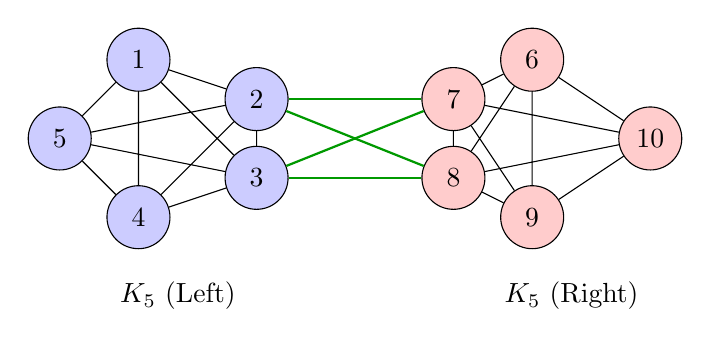
\begin{tikzpicture}[scale=1]
    % Left K_5 vertices
    \node[circle, fill=blue!20, draw, minimum size=8mm] (L1) at (0,2) {1};
    \node[circle, fill=blue!20, draw, minimum size=8mm] (L2) at (1.5,1.5) {2};
    \node[circle, fill=blue!20, draw, minimum size=8mm] (L3) at (1.5,0.5) {3};
    \node[circle, fill=blue!20, draw, minimum size=8mm] (L4) at (0,0) {4};
    \node[circle, fill=blue!20, draw, minimum size=8mm] (L5) at (-1,1) {5};
    
    % Right K_5 vertices
    \node[circle, fill=red!20, draw, minimum size=8mm] (R1) at (5,2) {6};
    \node[circle, fill=red!20, draw, minimum size=8mm] (R2) at (4,1.5) {7};
    \node[circle, fill=red!20, draw, minimum size=8mm] (R3) at (4,0.5) {8};
    \node[circle, fill=red!20, draw, minimum size=8mm] (R4) at (5,0) {9};
    \node[circle, fill=red!20, draw, minimum size=8mm] (R5) at (6.5,1) {10};
    
    % Left K_5 edges
    \draw (L1) -- (L2) -- (L3) -- (L4) -- (L5) -- (L1);
    \draw (L1) -- (L3) -- (L5) -- (L2) -- (L4) -- (L1);
    
    % Right K_5 edges
    \draw (R1) -- (R2) -- (R3) -- (R4) -- (R5) -- (R1);
    \draw (R1) -- (R3) -- (R5) -- (R2) -- (R4) -- (R1);
    
    % Cross-connections between the two specified vertices from each K_5
    % Let's say vertex 2 and 3 from left K_5 connect to vertices 7 and 8 from right K_5
    \draw[thick, color=green!60!black] (L2) -- (R2);
    \draw[thick, color=green!60!black] (L2) -- (R3);
    \draw[thick, color=green!60!black] (L3) -- (R2);
    \draw[thick, color=green!60!black] (L3) -- (R3);
    
    % Labels
    \node at (0.5,-1) {$K_5$ (Left)};
    \node at (5.5,-1) {$K_5$ (Right)};
    
\end{tikzpicture}
\end{figure}

\subsubsection*{A 3-connected graph that is not 2-connected}
No such example exists, since, by definition a 3-connected graph $G$ satisfies $\kappa(G) \ge 3 \ge 2$ making it also 2-connected

\subsubsection*{A 2-edge-connected graph that is not 3-edge-connected}
We are looking for a graph with $\lambda (G) = 2$

\begin{figure}[h]
\centering
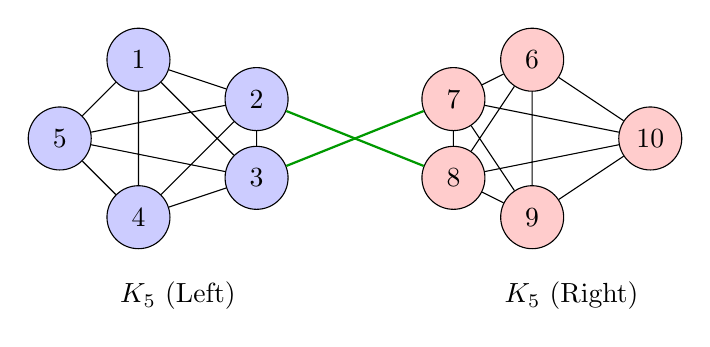
\begin{tikzpicture}[scale=1]
    % Left K_5 vertices
    \node[circle, fill=blue!20, draw, minimum size=8mm] (L1) at (0,2) {1};
    \node[circle, fill=blue!20, draw, minimum size=8mm] (L2) at (1.5,1.5) {2};
    \node[circle, fill=blue!20, draw, minimum size=8mm] (L3) at (1.5,0.5) {3};
    \node[circle, fill=blue!20, draw, minimum size=8mm] (L4) at (0,0) {4};
    \node[circle, fill=blue!20, draw, minimum size=8mm] (L5) at (-1,1) {5};
    
    % Right K_5 vertices
    \node[circle, fill=red!20, draw, minimum size=8mm] (R1) at (5,2) {6};
    \node[circle, fill=red!20, draw, minimum size=8mm] (R2) at (4,1.5) {7};
    \node[circle, fill=red!20, draw, minimum size=8mm] (R3) at (4,0.5) {8};
    \node[circle, fill=red!20, draw, minimum size=8mm] (R4) at (5,0) {9};
    \node[circle, fill=red!20, draw, minimum size=8mm] (R5) at (6.5,1) {10};
    
    % Left K_5 edges
    \draw (L1) -- (L2) -- (L3) -- (L4) -- (L5) -- (L1);
    \draw (L1) -- (L3) -- (L5) -- (L2) -- (L4) -- (L1);
    
    % Right K_5 edges
    \draw (R1) -- (R2) -- (R3) -- (R4) -- (R5) -- (R1);
    \draw (R1) -- (R3) -- (R5) -- (R2) -- (R4) -- (R1);
    
    % Cross-connections between the two specified vertices from each K_5
    % Let's say vertex 2 and 3 from left K_5 connect to vertices 7 and 8 from right K_5

    \draw[thick, color=green!60!black] (L2) -- (R3);
    \draw[thick, color=green!60!black] (L3) -- (R2);

    
    % Labels
    \node at (0.5,-1) {$K_5$ (Left)};
    \node at (5.5,-1) {$K_5$ (Right)};
    
\end{tikzpicture}
\end{figure}

\subsubsection*{A 3-edge-connected graph that is not 2-edge-connected}
No such example exists, since, by definition a 3-edge-connected graph $G$ satisfies $\lambda(G) \ge 3 \ge 2$ making it also 2-edge-connected

\newpage 
\subsubsection*{A graph $G$ with $\kappa (G) = 2, \lambda (G) = 3,$ and $\delta (G) = 4$}

\begin{figure}[h]
\centering
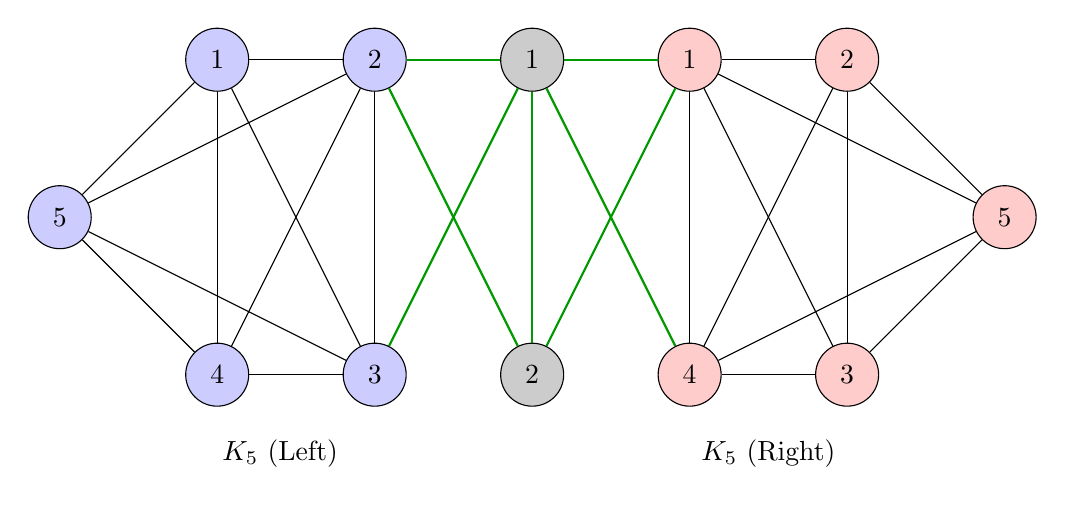
\begin{tikzpicture}[scale=1]
    % Left K_4 vertices
    \node[circle, fill=blue!20, draw, minimum size=8mm] (L1) at (0,4) {1};
    \node[circle, fill=blue!20, draw, minimum size=8mm] (L2) at (2, 4) {2};
    \node[circle, fill=blue!20, draw, minimum size=8mm] (L3) at (2, 0) {3};
    \node[circle, fill=blue!20, draw, minimum size=8mm] (L4) at (0,0) {4};
    \node[circle, fill=blue!20, draw, minimum size=8mm] (L5) at (-2,2) {5};
    
    % Middle connectors
    \node[circle, fill=black!20, draw, minimum size=8mm] (C1) at (4,4) {1};
    \node[circle, fill=black!20, draw, minimum size=8mm] (C2) at (4, 0) {2};
    
    % Right K_4 vertices
    \node[circle, fill=red!20, draw, minimum size=8mm] (R1) at (6, 4) {1};
    \node[circle, fill=red!20, draw, minimum size=8mm] (R2) at (8, 4) {2};
    \node[circle, fill=red!20, draw, minimum size=8mm] (R3) at (8, 0) {3};
    \node[circle, fill=red!20, draw, minimum size=8mm] (R4) at (6,0) {4};
    \node[circle, fill=red!20, draw, minimum size=8mm] (R5) at (10,2) {5};
    
    % Left K_4 edges
    \draw (L1) -- (L2) -- (L3) -- (L4) -- (L1);
    \draw (L1) -- (L3);
    \draw (L2) -- (L4);
    \draw (L5) -- (L1);
    \draw (L5) -- (L2);
    \draw (L5) -- (L3);
    \draw (L5) -- (L4);
    
    % Right K_4 edges
    \draw (R1) -- (R2) -- (R3) -- (R4) -- (R1);
    \draw (R1) -- (R3);
    \draw (R2) -- (R4);
    \draw (R5) -- (R1);
    \draw (R5) -- (R2);
    \draw (R5) -- (R3);
    \draw (R5) -- (R4);
    
    % Cross-connections between the two specified vertices from each K_5
    % Let's say vertex 2 and 3 from left K_5 connect to vertices 7 and 8 from right K_5

    \draw[thick, color=green!60!black] (L2) -- (C1) -- (R1);
    \draw[thick, color=green!60!black] (L2) -- (C2) -- (R1);
    \draw[thick, color=green!60!black] (L3) -- (C1) -- (R4);
    \draw[thick, color=green!60!black] (C1) -- (C2);

    
    % Labels
    \node at (0.8,-1) {$K_5$ (Left)};
    \node at (7,-1) {$K_5$ (Right)};
    
\end{tikzpicture}
\end{figure}

\subsubsection*{A graph $G$ with $\kappa (G) = 3, \lambda (G) = 2,$ and $\delta (G) = 4$}
This cannot happen due to Witney's Theorem.


\subsubsection*{A graph $G$ with $\kappa (G) = 3, \lambda (G) = 3,$ and $\delta (G) = 2$}

Again, this is impossible by Witney's Theorem

\subsubsection*{A graph $G$ with $\kappa (G) = 2, \lambda (G) = 2,$ and $\delta (G) = 3$}

\begin{figure}[h]
\centering
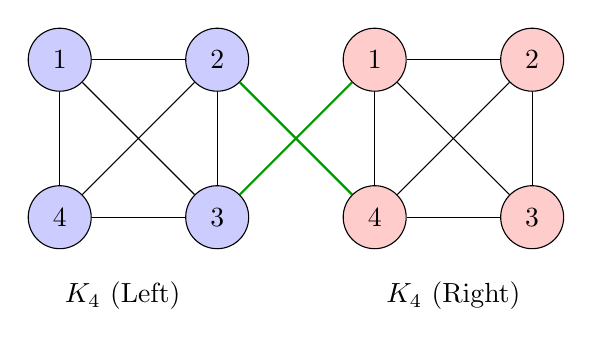
\begin{tikzpicture}[scale=1]
    % Left K_4 vertices
    \node[circle, fill=blue!20, draw, minimum size=8mm] (L1) at (0,2) {1};
    \node[circle, fill=blue!20, draw, minimum size=8mm] (L2) at (2, 2) {2};
    \node[circle, fill=blue!20, draw, minimum size=8mm] (L3) at (2, 0) {3};
    \node[circle, fill=blue!20, draw, minimum size=8mm] (L4) at (0,0) {4};
    

    
    % Right K_4 vertices
    \node[circle, fill=red!20, draw, minimum size=8mm] (R1) at (4, 2) {1};
    \node[circle, fill=red!20, draw, minimum size=8mm] (R2) at (6, 2) {2};
    \node[circle, fill=red!20, draw, minimum size=8mm] (R3) at (6, 0) {3};
    \node[circle, fill=red!20, draw, minimum size=8mm] (R4) at (4,0) {4};
    
    % Left K_4 edges
    \draw (L1) -- (L2) -- (L3) -- (L4) -- (L1);
    \draw (L1) -- (L3);
    \draw (L2) -- (L4);

    
    % Right K_4 edges
    \draw (R1) -- (R2) -- (R3) -- (R4) -- (R1);
    \draw (R1) -- (R3);
    \draw (R2) -- (R4);

    
    % Cross-connections between the two specified vertices from each K_5
    % Let's say vertex 2 and 3 from left K_5 connect to vertices 7 and 8 from right K_5

    \draw[thick, color=green!60!black] (L2) -- (R4);
    \draw[thick, color=green!60!black] (L3) -- (R1);
    

    
    % Labels
    \node at (0.8,-1) {$K_4$ (Left)};
    \node at (5,-1) {$K_4$ (Right)};
    
\end{tikzpicture}
\end{figure}

\newpage

\subsection*{Question 2: Prove that, for all positive integers $a,b,c$ with $a \le b \le c$, there is a connected graph $G$ with $\kappa (G) = a, \lambda (G) = b, $ and $\delta (G) = c$}
Start with 2 copies of $K_{c+1}$. Label the left vertices $x_1, ..., x_{c+1}$, the right $z_1, ..., z_{c+1}$. We first deal with $\kappa (G) = a$. Connect $x_i$ to $y_i$ for $1\le i \le a$. But $\lambda (G) = a$, so connect $x_a$ to each of $y_{a+1}, ..., y_{b}$, and this graph satisfies the criteria.
\begin{figure}[h]
\centering
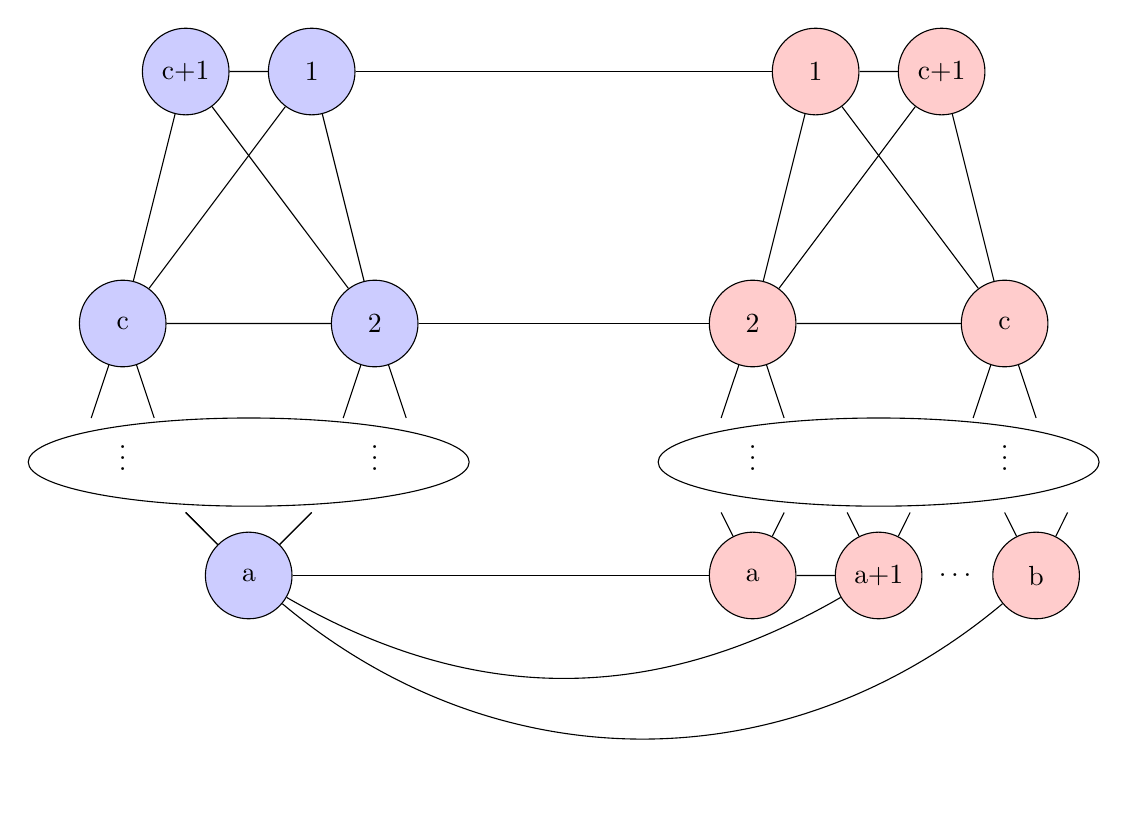
\begin{tikzpicture}[scale=0.8]
    % Left K_4 vertices
    \node[circle, fill=blue!20, draw, minimum size=11mm] (L1) at (-1,4) {c+1};
    \node[circle, fill=blue!20, draw, minimum size=11mm] (L2) at (1, 4) {1};
    \node[circle, fill=blue!20, draw, minimum size=11mm] (L3) at (2, 0) {2};
    \node[circle, fill=blue!20, draw, minimum size=11mm] (L4) at (-2,0) {c};
    

    
    % Right K_4 vertices
    \node[circle, fill=red!20, draw, minimum size=11mm] (R1) at (9,4) {1};
    \node[circle, fill=red!20, draw, minimum size=11mm] (R2) at (11, 4) {c+1};
    \node[circle, fill=red!20, draw, minimum size=11mm] (R3) at (12, 0) {c};
    \node[circle, fill=red!20, draw, minimum size=11mm] (R4) at (8,0) {2};
    
    \draw (L1) -- (L2) -- (L3) -- (L4) -- (L1);
    \draw (L3) -- (1.5, -1.5);
    \draw (L3) -- (2.5, -1.5);
    
     \draw (L4) -- (-2.5, -1.5);
     \draw (L4) -- (-1.5, -1.5);
     
     \draw (L1) -- (L3);
     \draw (L2) -- (L4);
    
      \node at (-2,-2) {$ \vdots $};
      \node at (2,-2) {$ \vdots $};    
      
	\node[circle, fill=blue!20, draw, minimum size=11mm] (L5) at (0,-4) {a};
	\draw (L5) -- (-1, -3);
	\draw (L5) -- (1, -3);
      
      
      \draw (R1) -- (R2) -- (R3) -- (R4) -- (R1);
    \draw (R3) -- (11.5, -1.5);
    \draw (R3) -- (12.5, -1.5);
    
     \draw (R4) -- (7.5, -1.5);
     \draw (R4) -- (8.5, -1.5);
     
     \draw (R1) -- (R3);
     \draw (R2) -- (R4);
    
      \node at (8,-2) {$ \vdots $};
      \node at (12,-2) {$ \vdots $}; 
      
      \draw (L2) -- (R1);
      \draw (L3) -- (R4);
      
      
      \node[circle, fill=red!20, draw, minimum size=11mm] (R5) at (8,-4) {a};
      \node[circle, fill=red!20, draw, minimum size=11mm] (R6) at (10,-4) {a+1};
	\draw (L5) -- (-1, -3);
	\draw (L5) -- (1, -3);
	
	\draw (R5) -- (R6);

	\draw (R5) -- (7.5, -3);
	\draw (R5) -- (8.5, -3);
	
	\draw (R6) -- (9.5, -3);
	\draw (R6) -- (10.5, -3);
	
	\draw (L5) -- (R5);
	\draw (L5) to[bend right=30] (R6);
	
	      \node at (11.25,-4) {$ \dots $}; 
	      
	  \node[circle, fill=red!20, draw, minimum size=11mm] (R7) at (12.5,-4) {b};
	  
	  	\draw (R7) -- (13, -3);
	\draw (R7) -- (12, -3);
	  
	  	\draw (L5) to[bend right=40] (R7);
		
		
		
\draw (0,-2.2) ellipse (3.5cm and 0.7cm);
\draw (10,-2.2) ellipse (3.5cm and 0.7cm);
	
        
    
\end{tikzpicture}
\end{figure}



\subsection*{Question 3: Prove that if $G$ is a graph of order $n$ such that $\delta (G) \ge (n-1)/2$, then $\lambda(G) = \delta(G)$}
We will first show $G$ is connected, and then by Witney's Theorem (although it extends to any graph, connectedness is needed for $\lambda (G)$), we will know that $\lambda(G) \leq \delta(G)$. Let $u$ and $v$ be any two vertices in $G$. If they are adjacent, they are connected. Assume they are non-adjacent. Since $\deg(u), \deg(v) \ge \delta(G) \geq \frac{n-1}{2}$, both $u$ and $v$ have at least $\frac{n-1}{2}$ neighbours. $u$ and $v$ have at most $n-2$ total possible neighbours (all other vertices). But $\deg(u) + \deg(v) \geq 2 \cdot \frac{n-1}{2} = n-1$, so $u$ and $v$ must share a common neighbour. Through this common neighbour, there is a $u-v$ path, making $G$ connected. \\ ~\\ 
Let $T$ be an edge-cut for $G$, splitting $G$ into components $A$ and $B$. So $n = |A| + |B|$. We cannot have $|A|, |B| \ge \frac{n+1}{2}$ so assume $|A| < \frac{n+1}{2}$. Let $v \in A$. Then $v$ has at most $|A|-1$ neighbours in $A$, and thus at least $\delta (G) - |A| + 1$ neighbours in $B$. Then the number of removed edges \[|T| \ge \sum \limits _{v \in A} (\delta (G) - |A| + 1) = |A| (\delta (G) - |A| + 1)\]Now \[
|A|(\delta (G) - |A| + 1) \ge \delta (G) \iff \delta (G) \left [ |A| - 1\right ] \ge |A| \left [ |A| - 1\right ]\] The case $|A| = 1$ proves this trivially. Otherwise we consider 2 cases: 
\begin{enumerate}
	\item $n$ is even. Then $n = 2a, a \in \mathbb{N}$ and $|A| <  \frac{2a + 1}{2}$, and because $|A|$ is an integer, $|A| \le a$. We have that $\delta (G) \ge (2a-1)/2$, and since it is an integer, $\delta (G) \ge a$ as required.
	\item $n$ is odd. Then $n = 2a + 1, a \in \mathbb{N}$ and $|A| < \frac{2a + 2}{2} = a+1$. So $|A| \le a$. We have that $\delta (G) \ge (2a)/2 = a$, as required.
	

\end{enumerate}
In all cases, $\delta (G) \ge |A|$ and so $|T| \ge \delta (G)$. This is for any edge-cut, so $\lambda (G) \ge \delta (G)$. Finally, $\delta (G) = \lambda (G)$ \subsection*{Question 4. Determine the connectivity and edge-connectivity of:}

\subsubsection*{The Petersen Graph}

\begin{figure}[h]
\centering
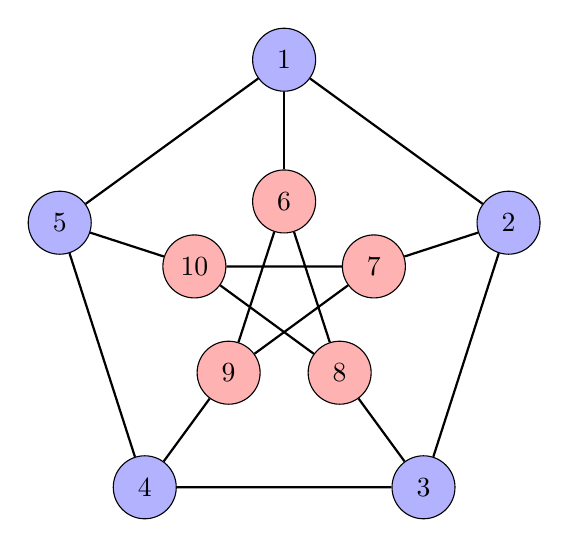
\begin{tikzpicture}[scale=1.5]
    % Outer pentagon vertices
    \node[circle, fill=blue!30, draw, minimum size=8mm] (O1) at (0,2) {1};
    \node[circle, fill=blue!30, draw, minimum size=8mm] (O2) at (1.9,0.62) {2};
    \node[circle, fill=blue!30, draw, minimum size=8mm] (O3) at (1.18,-1.62) {3};
    \node[circle, fill=blue!30, draw, minimum size=8mm] (O4) at (-1.18,-1.62) {4};
    \node[circle, fill=blue!30, draw, minimum size=8mm] (O5) at (-1.9,0.62) {5};
    
    % Inner pentagram vertices
    \node[circle, fill=red!30, draw, minimum size=8mm] (I1) at (0,0.8) {6};
    \node[circle, fill=red!30, draw, minimum size=8mm] (I2) at (0.76,0.25) {7};
    \node[circle, fill=red!30, draw, minimum size=8mm] (I3) at (0.47,-0.65) {8};
    \node[circle, fill=red!30, draw, minimum size=8mm] (I4) at (-0.47,-0.65) {9};
    \node[circle, fill=red!30, draw, minimum size=8mm] (I5) at (-0.76,0.25) {10};
    
    % Outer pentagon edges
    \draw[thick] (O1) -- (O2) -- (O3) -- (O4) -- (O5) -- (O1);
    
    % Inner pentagram edges (connecting every other vertex)
    \draw[thick] (I1) -- (I3) -- (I5) -- (I2) -- (I4) -- (I1);
    
    % Spokes connecting outer to inner
    \draw[thick] (O1) -- (I1);
    \draw[thick] (O2) -- (I2);
    \draw[thick] (O3) -- (I3);
    \draw[thick] (O4) -- (I4);
    \draw[thick] (O5) -- (I5);
    
\end{tikzpicture}
\caption{The Petersen Graph}
\label{fig:petersen}
\end{figure}
~\\ $\kappa (G) = 3$, so $G$ is $k$-connected for $k \le 3$. We can prove this easily with Menger's Theorem, where if $u$ and $v$ are both external and non-adjacent (we cannot separate adjacent vertices with vertex-cuts), $\kappa(u, v) = p(u,v) = 3$ (two outside the hexagon using all sides, and one inside). If one is external, one is internal, again, we have the direct path going through the middle, and two around the hexagon. If two are internal, we have the one inside the hexagon and two outside. Then $\kappa (G) = \min \limits _{u,v \in G} \kappa (u,v) = 3$. \\ ~\\ Since $\delta (G) = 3$, by Witney's Theorem, $\lambda (G) = 3$. Alternatively, note that every vertex has degree $3$, and even if we remove 2 edges, we can reach every vertex from every other vertex, so we must remove 3 edges at least, with 3 being obtained isolating vertex 4 for example. 

\subsubsection*{The $t$-cube $Q_t$}

% Hypercubes Q_1 through Q_4 in minipages
\begin{figure}[h]
\centering
\begin{minipage}{0.12\textwidth}
\centering
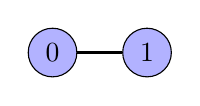
\begin{tikzpicture}[scale=0.8]
    \node[circle, fill=blue!30, draw, minimum size=6mm] (v0) at (0,0) {0};
    \node[circle, fill=blue!30, draw, minimum size=6mm] (v1) at (1.5,0) {1};
    \draw[thick] (v0) -- (v1);
\end{tikzpicture}
\caption{$Q_1$}
\end{minipage}%
\hfill
\begin{minipage}{0.12\textwidth}
\centering
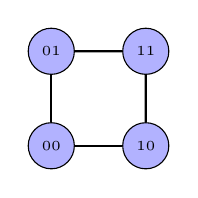
\begin{tikzpicture}[scale=0.8]
    \node[circle, fill=blue!30, draw, minimum size=5mm] (v00) at (0,0) {\tiny 00};
    \node[circle, fill=blue!30, draw, minimum size=5mm] (v01) at (0,1.5) {\tiny 01};
    \node[circle, fill=blue!30, draw, minimum size=5mm] (v10) at (1.5,0) {\tiny 10};
    \node[circle, fill=blue!30, draw, minimum size=5mm] (v11) at (1.5,1.5) {\tiny 11};
    
    \draw[thick] (v00) -- (v01);
    \draw[thick] (v00) -- (v10);
    \draw[thick] (v01) -- (v11);
    \draw[thick] (v10) -- (v11);
\end{tikzpicture}
\caption{$Q_2$}
\end{minipage}%
\hfill
\begin{minipage}{0.3\textwidth}
\centering
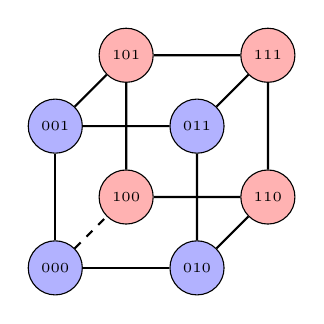
\begin{tikzpicture}[scale=1.5]
    % Front face vertices
    \node[circle, fill=blue!30, draw, minimum size=4mm] (v000) at (0,0) {\tiny 000};
    \node[circle, fill=blue!30, draw, minimum size=4mm] (v001) at (0,1.2) {\tiny 001};
    \node[circle, fill=blue!30, draw, minimum size=4mm] (v010) at (1.2,0) {\tiny 010};
    \node[circle, fill=blue!30, draw, minimum size=4mm] (v011) at (1.2,1.2) {\tiny 011};
    
    % Back face vertices (shifted for 3D effect)
    \node[circle, fill=red!30, draw, minimum size=4mm] (v100) at (0.6,0.6) {\tiny 100};
    \node[circle, fill=red!30, draw, minimum size=4mm] (v101) at (0.6,1.8) {\tiny 101};
    \node[circle, fill=red!30, draw, minimum size=4mm] (v110) at (1.8,0.6) {\tiny 110};
    \node[circle, fill=red!30, draw, minimum size=4mm] (v111) at (1.8,1.8) {\tiny 111};
    
    % Front face edges
    \draw[thick] (v000) -- (v001);
    \draw[thick] (v000) -- (v010);
    \draw[thick] (v001) -- (v011);
    \draw[thick] (v010) -- (v011);
    
    % Back face edges
    \draw[thick] (v100) -- (v101);
    \draw[thick] (v100) -- (v110);
    \draw[thick] (v101) -- (v111);
    \draw[thick] (v110) -- (v111);
    
    % Connecting edges (front to back)
    \draw[thick, dashed] (v000) -- (v100);
    \draw[thick] (v001) -- (v101);
    \draw[thick] (v010) -- (v110);
    \draw[thick] (v011) -- (v111);
\end{tikzpicture}
\caption{$Q_3$}
\end{minipage}%
\hfill
\begin{minipage}{0.35\textwidth}
\centering
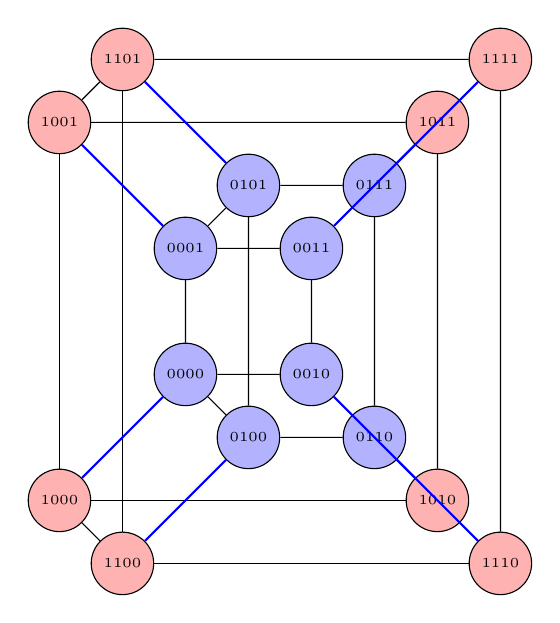
\begin{tikzpicture}[scale=1.6]
    % Inner cube vertices
    \node[circle, fill=blue!30, draw, minimum size=3mm] (v0000) at (1,1) {\tiny 0000};
    \node[circle, fill=blue!30, draw, minimum size=3mm] (v0001) at (1,2) {\tiny 0001};
    \node[circle, fill=blue!30, draw, minimum size=3mm] (v0010) at (2,1) {\tiny 0010};
    \node[circle, fill=blue!30, draw, minimum size=3mm] (v0011) at (2,2) {\tiny 0011};
    \node[circle, fill=blue!30, draw, minimum size=3mm] (v0100) at (1.5,0.5) {\tiny 0100};
    \node[circle, fill=blue!30, draw, minimum size=3mm] (v0101) at (1.5,2.5) {\tiny 0101};
    \node[circle, fill=blue!30, draw, minimum size=3mm] (v0110) at (2.5,0.5) {\tiny 0110};
    \node[circle, fill=blue!30, draw, minimum size=3mm] (v0111) at (2.5,2.5) {\tiny 0111};
    
    % Outer cube vertices
    \node[circle, fill=red!30, draw, minimum size=3mm] (v1000) at (0,0) {\tiny 1000};
    \node[circle, fill=red!30, draw, minimum size=3mm] (v1001) at (0,3) {\tiny 1001};
    \node[circle, fill=red!30, draw, minimum size=3mm] (v1010) at (3,0) {\tiny 1010};
    \node[circle, fill=red!30, draw, minimum size=3mm] (v1011) at (3,3) {\tiny 1011};
    \node[circle, fill=red!30, draw, minimum size=3mm] (v1100) at (0.5,-0.5) {\tiny 1100};
    \node[circle, fill=red!30, draw, minimum size=3mm] (v1101) at (0.5,3.5) {\tiny 1101};
    \node[circle, fill=red!30, draw, minimum size=3mm] (v1110) at (3.5,-0.5) {\tiny 1110};
    \node[circle, fill=red!30, draw, minimum size=3mm] (v1111) at (3.5,3.5) {\tiny 1111};
    
    % Inner cube edges
    \draw (v0000) -- (v0001);
    \draw (v0000) -- (v0010);
    \draw (v0000) -- (v0100);
    \draw (v0001) -- (v0011);
    \draw (v0001) -- (v0101);
    \draw (v0010) -- (v0011);
    \draw (v0010) -- (v0110);
    \draw (v0011) -- (v0111);
    \draw (v0100) -- (v0101);
    \draw (v0100) -- (v0110);
    \draw (v0101) -- (v0111);
    \draw (v0110) -- (v0111);
    
    % Outer cube edges
    \draw (v1000) -- (v1001);
    \draw (v1000) -- (v1010);
    \draw (v1000) -- (v1100);
    \draw (v1001) -- (v1011);
    \draw (v1001) -- (v1101);
    \draw (v1010) -- (v1011);
    \draw (v1010) -- (v1110);
    \draw (v1011) -- (v1111);
    \draw (v1100) -- (v1101);
    \draw (v1100) -- (v1110);
    \draw (v1101) -- (v1111);
    \draw (v1110) -- (v1111);
    
    % Connecting edges between cubes
    \draw[thick, blue] (v0000) -- (v1000);
    \draw[thick, blue] (v0001) -- (v1001);
    \draw[thick, blue] (v0010) -- (v1010);
    \draw[thick, blue] (v0011) -- (v1011);
    \draw[thick, blue] (v0100) -- (v1100);
    \draw[thick, blue] (v0101) -- (v1101);
    \draw[thick, blue] (v0110) -- (v1110);
    \draw[thick, blue] (v0111) -- (v1111);
\end{tikzpicture}
\caption{$Q_4$}
\end{minipage}
\end{figure}
~\\
Note that from each vertex, in binary $x_1x_2...x_t$, we can travel to any other node that changes exactly one binary digit. 
Let $u,v$ be two vertices in binary form. We want to show $p(u,v) = t$. If $v$ is the destination vertex, there are $t$ paths into $v$ (one for each binary digit). So we just have to show there is a path for each of these edges, and these paths are disjoint. Comparing $u$ and $v$,  let $F$ be the indices that are the same, and $D$ different. There are exactly $|D|$ paths that only using the differing digits, by choosing one digit as the end edge, and work backwards choosing only vertices in $D$. We can choose this unique by first processing all digits less than (in order) and cycling around doing the largest down. Mathematically, if we let $d_1, ..., d_{|D|}$ be the differences and $\bar{d}_i$ represents flipping that digit. Consider starting with digit $i$ and $j$, for $i \ne j$. We will show that the state will never be the same. Without loss of generality, assume $i > j$. \\ Then consider step $k \le j$: (steps being how many changes we have processed, starting at $i$ or $j$) \\~
\\For starting with $i$, we are in state $d_1 ... \bar{d}_{i-k+1} \dots \bar{d}_j \dots \bar{d}_i d_{i+1} \dots d_{|D|}$. 
\\For starting with $j$, we are in state $d_1 ... \bar{d}_{j-k+1} \dots \bar{d}_j  d_{j+1} \dots d_{|D|}$.  
\\~\\and they clearly differ at $d_i$. Consider step $k = j + 1$ (wraparound for $j$). \\~
\\For starting with $i$,we are in state $d_1 ... \bar{d}_{i-k+1} \dots \bar{d}_j \dots \bar{d}_i d_{i+1} \dots d_{|D|}$. 
\\For starting with $j$, we are in state $\bar{d}_1 ... \bar{d}_j  d_{j+1} \dots d_{|D|}$.  
\\ ~\\and they clearly differ at $d_i$ again. After the wraparound, for $i \ge k > j$, \\~
\\For starting with $i$, we are in state $d_1 ... \bar{d}_{i-k+1} \dots \bar{d}_j \dots \bar{d}_i d_{i+1} \dots d_{|D|}$. 
\\For starting with $j$, we are in state $\bar{d}_1 ... \bar{d}_j  d_{j+1} \dots d_{|D| - k + j} \bar{d}_{|D| - k + j + 1)} \dots \bar{d}_{|D|}$.  \\ ~\\and they differ at $d_{|D|}$. When $i$ wraps around, they differ at $d_{|D| - k + j + 1)} $ all the way until all digits are changed. \\ ~\\
Similarly, for each fixed digit, we first flip that, then process the differences, and then return from the flipped digit. (and these paths are guaranteed unique by that flipped fixed digit). This gives $|F|$ paths. The total is then $t$ paths. So $\kappa (G) = t$. Again, since $\delta (G) = t$, we get $\lambda (G) = t$


\subsubsection*{The Octahedron $\bar{K}_2 + C_4$}
\begin{center}
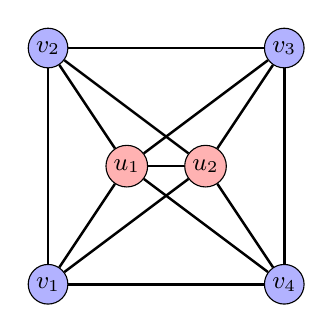
\begin{tikzpicture}[
    every node/.style={circle, draw, inner sep=1.6pt, minimum size=10pt, font=\small},
    c4/.style={circle, fill=blue!30, draw, minimum size=3mm},
    k2/.style={circle, fill=red!30, draw, minimum size=3mm},
    ed/.style={line width=0.9pt}
  ]
  
  

  % C4 vertices (square)
  \node[c4] (v1) at (0,0)  {$v_1$};
  \node[c4] (v2) at (0,3)  {$v_2$};
  \node[c4] (v3) at (3,3) {$v_3$};
  \node[c4] (v4) at (3,0) {$v_4$};

  % K2 vertices (to the right)
  \node[k2] (u1) at (1,1.5) {$u_1$};
  \node[k2] (u2) at (2,1.5){$u_2$};

  % Edges of C4 (cycle)
  \draw[ed] (v1) -- (v2) -- (v3) -- (v4) -- (v1);

  % Edge of K2
  \draw[ed] (u1) -- (u2);

  % Join edges (use different bends to avoid clutter)
  \draw[ed] (u1) --  (v1);
  \draw[ed] (u1) --  (v2);
  \draw[ed] (u1) --  (v3);
  \draw[ed] (u1) -- (v4);

  \draw[ed] (u2) -- (v1);
  \draw[ed] (u2) -- (v2);
  \draw[ed] (u2) --  (v3);
  \draw[ed] (u2) --  (v4);


\end{tikzpicture}
\end{center}
If $u$ and $v$ are vertices, both part of $C_4$, the 4 paths are: around left, around right, through $u_1$, through $u_2$. This is the only case with non-adjacent vertices, so $\kappa (G) = 4$. Again, $\delta (G) = 4$ so $\lambda (G) = 4$. If we try directly, notice vertex cuts involve isolating $v_2$ from $v_4$ or $v_1$ from $v_3$, and then clearly 4 must be removed.

\subsection*{Question 5: Prove that if $G$ is a $k$-connected graph of order $n$ and size $m$, then $m \ge \frac{1}{2}kn$}
Note that $\kappa (G) \ge k$, so $\delta (G) \ge k$. By the Handshaking Lemma, \[
2m = \sum \limits _{v \in G} \deg v \ge \sum \limits _{v\in G} k = kn \Longrightarrow m \ge \frac{1}{2}kn
\]

\subsection*{Question 6: Prove that if $G$ is a $k$-connected graph and $e$ is an edge of $G$, then $G-e$ is $(k-1)$-connected}
$G$ is $k$-connected, so $\kappa (G) \ge k$. Let edge $e = uv$ and $P$ be a vertex-cut of $G-e$. Then if either $u$ or $v$ is in $P$, it is also a vertex-cut for $G$ and so $|P| \ge k$ If not, we have 2 cases. If $T$ is every vertex except $u$ and $v$, it removes all of $u$'s neighbours except $v$, and so $|T| \ge \deg v - 1 \ge \delta (G) - 1\ge \kappa (G) - 1 \ge k-1 $. Otherwise, $P \cup \{u\}$ is a vertex-cut of $G$. To prove this, since $P$ is a vertex-cut and not every other vertex, we have some $x \ne u, x \ne v$ in a different component to some other $y$ (maybe $u$ or $v$, without loss of generality assume it is $v$ if it is one of these). Then, cutting $P \cup \{u\}$ removes edge $e$, and thus separates $x$ and $y$. Thus $|P \cup \{u\}| \ge k$, that is, $|P| \ge k-1$. So $G-e$ is $(k-1)$-connected

 \subsection*{Question 7: Prove or disprove: If $k$ is a positive integer, then $k - \lceil \frac{k}{2} \rceil= \lfloor \frac{k}{2}\rfloor$}             
 This is true, and to prove it, we consider 2 cases:
 \begin{enumerate}
 \item $k$ is even. Then $k = 2a$ for some $a \in \mathbb{N}$ and thus $k - \lceil \frac{k}{2} \rceil = 2a - \lceil \frac{2a}{2} \rceil = 2a-a = a = \lfloor \frac{2a}{2}\rfloor$
 \item $k$ is odd. Then $k = 2a + 1$ for some $a \in \mathbb{N}$ and thus $k - \lceil \frac{k}{2} \rceil = 2a + 1 - \lceil \frac{2a+1}{2} \rceil = 2a + 1 - \lceil a + \frac{1}{2} \rceil = 2a+1-(a+1) = a$ and $\lfloor \frac{2a+1}{2}\rfloor  = \lfloor a+ \frac{1}{2}\rfloor  = a$ 
 \end{enumerate}
 So for every positive integer, $k - \lceil \frac{k}{2} \rceil= \lfloor \frac{k}{2}\rfloor$

\subsection*{Question 8: Prove or disprove: If $a$ and $b$ are integers, then $\lfloor (b-a)/2 \rfloor + a = \lfloor (b+a)/2 \rfloor $ }             
This is true.  We will first show that $\lfloor x \rfloor + n = \lfloor x+n \rfloor$ for integers $n$ and real numbers $x$. Note that $x = \lfloor x \rfloor + r$ for some $r \in [0,1)$ (specifically, $r = x - \lfloor x \rfloor$). Then $x+n = \underbrace{(\lfloor x \rfloor + n)}_{\in \mathbb{Z}} + r$ and thus $\lfloor x +n \rfloor = \lfloor x \rfloor + n$ as required. Applying this to our problem, we get $\lfloor (b-a)/2 \rfloor + a = \lfloor (b-a)/2 + a \rfloor = \lfloor (b+a)/2 \rfloor $

\subsection*{Question 9: Let $v_1, v_2, ..., v_k$ be $k$ distinct vertices of a $k$-connected graph $G$, and let $H$ be the graph formed from $G$ by introducing a new vertex $x$ and joining $x$ to all vertices $v_1, ..., v_k$. Prove that $\kappa (H) = k$} 
First note that $\kappa (G) \ge k$. Let $T$ be a vertex-cut for $H$. If $x\in T$, then $T \setminus \{x\}$ is a vertex cut for $H $, so $|V \setminus \{x\}| \ge k$ and so $|V| \ge k$. If $x \not \in V$, suppose $H$ is cut into components $C_1, ..., C_N$ and, without loss of generality, assume $x \in C_1$. We have 2 cases: 
\begin{enumerate}
	\item $|C_1| = 1$. Then every vertex $v_1, ..., v_k$ has been cut and $|T| \ge k$.
	\item $|C_1| \ne 1$. Then there exists some vertex $v_i$ that has not been cut, and $T$ is also a vertex-cut for $G$. To prove this,  $v_i$ is separated from some other vertex $u \in V(G)$. If they are not separated in $G$ when cutting $T$, the path between them is also a path in $H$. So $T$ is a vertex-cut in $G$ and $|T| \ge k$.
	\end{enumerate}
So $|V| \ge k$ for any vertex-cut $T$. Considering the vertex-cut $\{v_1, ..., v_k\}$ (isolating $x$), we get $\kappa (H) = k$.

\subsection*{Question 10: Prove The Fan Lemma}

Consider the graph $H$ obtained by adding a new vertex $x$, and adding the edges $xv_1, ..., xv_k$. By Question 9, this graph is $k$-connected. So there exists at least $k$ internally disjoint $u-x$ paths. But $x$ is only neighbouring $k$ vertices, so there are exactly $k$ internally disjoint paths, each going through exactly one $v_i$ for $1 \le i \le k$. Considering these paths wtihout the final edge $v_ix$, we get internally disjoint paths where each $P_i$ is a $u-v_i$ path, as required

\subsection*{Question 11: Let $G$ be a $k$-connected graph of order $n \ge 2k$. Let $S_1$ and $S_2$ be two disjoint $k$-subsets of $V(G)$. Prove that $G$ contains $k$ disjoint (i.e. having no vertices in common) paths, each of which begins at a vertex in $S_1$ and ends at a vertex in $S_2$.}
Let $S_1 = \{v_1, ..., v_k\}$ and $S_2 = \{u_1, ..., u_k\}$. Consider modifying the graph $G$ into the graph $H$, by adding a vertex $x$, and, for all $v \in S_1$, adding the edge $xv$. By Question 9, this graph is $k$-connected. By the Fan Lemma, there exists paths $P_1, ..., P_k$ such that for all $i \in \{1,...,k\}$, $P_i$ is an $x-u_i$ path and the paths $P_1, P_2, ..., P_k$ are internally disjoint. So they only share the vertex $x$, and by considering the path removing the edges $xv_i$ for each $1\le i\le n$, we get the desired result.

\subsection*{Question 12: If $G$ is a connected cubic graph, prove that $\kappa (G) = \lambda (G)$}
By Witney's Theorem, $\kappa (G) \le \lambda (G) \le \delta (G) = 3$. We consider the different cases for $\kappa (G):$
\begin{itemize}
	\item $\kappa (G) = 1$:  \\ 
	\begin{center}
	\begin{tikzpicture}[
    vertex/.style={circle, draw, fill=white, inner sep=2pt},
    bridge/.style={thick, red},
    section/.style={circle, draw,, black, minimum size=3cm},
    edge/.style={thick, black}
]


\node[section] at (-3,0) {};
\node[vertex] (bridge) at (0, 0) {};
\node[section] at (3,0) {};

\draw (-1.56, 0.4) -- (bridge);
\draw (-1.56, -0.4) -- (bridge);
\draw (bridge) -- (1.5, 0);

\node[blue, above] at (0.74, 0) {\small $u$};


\end{tikzpicture}
\end{center}
We can remove edge $e$ and this shows $\lambda (G) = 1$

\item $\kappa (G) = 2$: We have 3 cases \\

\begin{minipage}{0.3\textwidth}
	\begin{center}
	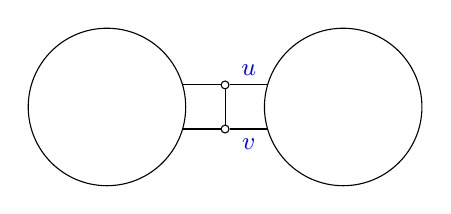
\begin{tikzpicture}[
    vertex/.style={circle, draw, fill=white, inner sep=1pt},
    bridge/.style={thick, red},
    section/.style={circle, draw,, black, minimum size=2cm},
    edge/.style={thick, black}
]


\node[section] at (-2,0) {};
\node[vertex] (bridge1) at (-0.5, 0.28) {};
\node[vertex] (bridge2) at (-0.5, -0.28) {};
\node[section] at (1,0) {};

\draw (-1.56/3*2, 0.28) -- (bridge1);
\draw (-1.56/3*2, -0.28) -- (bridge2);
\draw (bridge1) -- (0.04, 0.28);
\draw (bridge2) -- (0.04, -0.28);
\draw (bridge1) -- (bridge2);

\node[blue, above] at (-0.2, 0.28) {\small $u$};
\node[blue, below] at (-0.2, -0.28) {\small $v$};


\end{tikzpicture}
\end{center}
\end{minipage}%
\hfill%
\begin{minipage}{0.3\textwidth}
	\begin{center}
	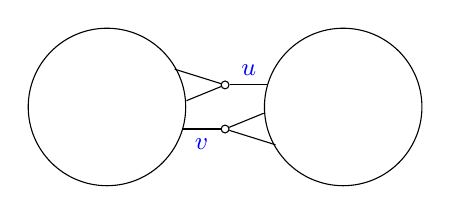
\begin{tikzpicture}[
    vertex/.style={circle, draw, fill=white, inner sep=1pt},
    bridge/.style={thick, red},
    section/.style={circle, draw,, black, minimum size=2cm},
    edge/.style={thick, black}
]


\node[section] at (-2,0) {};
\node[vertex] (bridge1) at (-0.5, 0.28) {};
\node[vertex] (bridge2) at (-0.5, -0.28) {};
\node[section] at (1,0) {};

\draw (-1.56/3*2+0.05, 0.08) -- (bridge1);
\draw (-1.56/3*2-0.1, 0.48) -- (bridge1);
\draw (-1.56/3*2, -0.28) -- (bridge2);
\draw (bridge1) -- (0.04, 0.28);

\draw (bridge2) -- (0.04-0.05, -0.08);
\draw (bridge2) -- (0.04+0.1, -0.48);


\node[blue, above] at (-0.2, 0.28) {\small $u$};
\node[blue, below] at (-0.8, -0.28) {\small $v$};


\end{tikzpicture}
\end{center}
\end{minipage}%
\hfill%
\begin{minipage}{0.3\textwidth}
	\begin{center}
	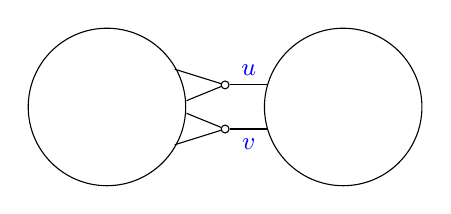
\begin{tikzpicture}[
    vertex/.style={circle, draw, fill=white, inner sep=1pt},
    bridge/.style={thick, red},
    section/.style={circle, draw,, black, minimum size=2cm},
    edge/.style={thick, black}
]


\node[section] at (-2,0) {};
\node[vertex] (bridge1) at (-0.5, 0.28) {};
\node[vertex] (bridge2) at (-0.5, -0.28) {};
\node[section] at (1,0) {};

\draw (-1.56/3*2+0.05, 0.08) -- (bridge1);
\draw (-1.56/3*2-0.1, 0.48) -- (bridge1);

\draw (-1.56/3*2+0.05, -0.08) -- (bridge2);
\draw (-1.56/3*2-0.1, -0.48) -- (bridge2);

\draw (bridge1) -- (0.04, 0.28);
\draw (bridge2) -- (0.04, -0.28);

\node[blue, above] at (-0.2, 0.28) {\small $u$};
\node[blue, below] at (-0.2, -0.28) {\small $v$};


\end{tikzpicture}
\end{center}
\end{minipage}


We can remove edges $u,v$ and this shows $\lambda (G) = 2$

\item $\kappa (G) = 3$. Then $3 = \kappa (G) \le \lambda (G) \le \delta (G) = 3$ so $\lambda (G) = 3$
\end{itemize}

\newpage

\subsection*{Question 13: If $G$ is a $k$-connected graph of order $n$, prove that $\text{diam } G \le \frac{n-2}{k} + 1$}
Take $u \in V$, and consider the sets $L_i := \{v \in V: d(u,v) = i\}$ for $i \in \mathbb{N}$. Let $d = e(u)$. Clearly then $L_i = \emptyset$ if $i > d$, and $L_0 = \{u\}$. Now we will show that if $|L_i| \ge k$ for all $1 \le i \le d-1$. If, to the contrary, that $|L_{i}| < k$ for some $1 \le i \le d-1$, then, considering $L_i$ as a vertex-cut, this will cut graph $G$ into at least 2 components, one with $u$, and one with a vertex from $L_d \ne \emptyset$. This then contradicts that $\kappa (G) \ge k$. So $|L_i| \ge k$ for $1 \le i \le d-1$. Clearly every vertex appears in only one $L_i$, so \[
n = \sum \limits _{i=1}^d |L_i| = |L_0| + |L_d| + \sum \limits _{i=1}^{d-1} |L_i| \ge 1 + 1 + \sum \limits _{i=1}^{d-1} k = 2+ (d-1)k
\]
Then \[
d \le \frac{n-2}{k} + 1
\]
So $e(u) \le \frac{n-2}{k} + 1$ for every vertex $u$, and thus $\text{diam }G \le \frac{n-2}{k} + 1$

\subsection*{Question 14: Determine $\kappa (K_{a,b})$}
Let $S_1$ be the set of $a$ vertices, and $S_2$ the set of $b$ vertices. As long as $S_1 \ne \emptyset$ and $S_2 \ne \emptyset$, this graph is connected. We show this now. Take $u,v \in G$. If $u \in S_1$ and $v \in S_2$, they are adjacent. If $u,v \in S_1$, there is some $w \in S_2$ and $u$ and $v$ are connected via vertex $w$. The case $u,v \in S_2$ and $u \in S_2, v \in S_1$ follow similarly. Thus, to create a vertex-cut we must remove at least $\min \{a,b\}$ vertices, and the vertex-cut removing entirely $S_1$ or $S_2$, whichever has $\min \{a,b\}$ vertices, achieves this, so $\kappa (K_{a,b}) = \min \{a,b\}$

\subsection*{Question 15: Is the converse of the Győri-Lovász Theorem true? (i.e., is it true that if $G$ has order $n$, then $G$ is $k$-connected if and only if whenever $v_1,v_2,...,v_k$ are distinct vertices of $G$ and $n_1,n_2,...,n_k$ are positive integers with $n_1+n_2+...+n_k = n$, then there are disjoint connected subgraphs $G_1, G_2, ..., G_k$ of $G$ such that for each $i \in [1,k]$ we have $v_i \in V(G_i)$ and $G_i$ has $n_i$ vertices}
The converse is not true. Consider the graph \\ 
% Minimal version - just the graph
\begin{center}
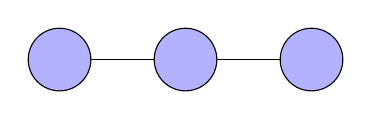
\begin{tikzpicture}[
    vertex/.style={circle, draw, fill=blue!30, minimum size=6pt, inner sep=8pt},
    bridge/.style={thick, red},
    scale=0.8
]

% Triangle 1
\node[vertex] (v1) at (0,0) {};
\node[vertex] (a1) at (2,0) {};
\node[vertex] (a2) at (4,0) {};
\draw (v1) -- (a1) -- (a2);


\end{tikzpicture}
\end{center}
Suppose that if $v_1, v_2, v_3$ are distinct vertices, and $n_1, n_2, n_3$ are positive integers with $n_1+n_2 +n_3= 3$, then there are disjoint connected subgraphs $G_1, G_2, G_3$ of $G$ such that for each $i=1,2,3$, we have $v_i \in V(G_i)$ and $G_i$ has $n_i$ vertices. We show that this implication holds in this graph. Clearly, since we only have 3 vertices, each vertex is used and we simply consider the subgraph of only that vertex. This implication holds but this graph is not 3-connected.
\end{document}
